\documentclass{article}
\usepackage[pdftex]{graphicx}
\graphicspath{{../images/}}
\usepackage{boxedminipage}
\usepackage[hints]{ms}
\usepackage{tikz}
\usepackage{url}
\usepackage[utf8]{inputenc}
\begin{document}
\begin{titlebox}{Exploring Cluster Data}
Ilaria Caiazzo, Jeremy Heyl \\
TAs: Xianfei Zhang, Sarafina Nance, Ilka Petermann
\end{titlebox}

\section{Introduction}

Globular clusters are groups of up to one million or more stars that were born at nearly the same time, with approximately the same composition and lie at a common distance from us.  This means that by today, the main parameter that will determine how the stars will appear is their mass. To understand the population one must determine the shared age, distance and composition of the group of stars. These properties of globular clusters (and open clusters as well) make them powerful laboratories to understand stellar evolution and test new physics.

\section{The Inlist}

We will start with the \texttt{test\_suite} directory \texttt{1M\_pre\_ms\_to\_wd} and change it for our initial models.  We will assign each student an initial mass and initial metallicity to run and we will bring together all of the data in the next laboratory ``Translating MESA Results to Observables.'' Here is the list of models:

\begin{center}
\begin{tabular}{c|ccc}
\hline
M+0.00 &
M-0.50 &
M-1.00 &
M-1.50 
\\
\hline
$Z=0.02$ &
$Z=0.007$ &
$Z=0.002$ & 
$Z=0.0007$ 
\\  
\hline 
3.0 & 1.1 & 1.1 & 1.1  \\
2.1 & 0.8 & 0.8 & 0.8  \\
1.5 & 0.6 & 0.6 & 0.6 \\
1.1 & 0.4 & 0.4 & 0.4  \\
0.8 & 0.3 & 0.3 & 0.3  \\
0.6 & 0.21 & 0.21 & 0.21 \\
0.4 & 0.15 & 0.15 & 0.15 \\
0.3 & 0.11 & 0.11 & 0.11 
\end{tabular}
\end{center}

Typically it takes MESA only a few minutes to reach the end of the central hydrogen burning but at least an hour to start helium burning and ascend the asymptotic giant branch, so if you start the models now, we will have a suite of models reaching up the giant branch and perhaps into the helium-burning regime.

{\bf Task:}
\begin{enumerate}
 \setlength\itemsep{0em}
    \item 
Set \texttt{initial\_mass} and \texttt{initial\_z} equal to your assigned values in the table.  
\item Add  \texttt{envelope\_fraction\_left\_limit = 0.05} and  \texttt{max\_age = 1.3ed10} in the \texttt{star\_controls} section of the \texttt{inlist} file.
\item Change \texttt{logL\_lower\_limit} from $-1$ to $-6$.
\item Make and run MESA.
\item When you model is complete, please upload the \texttt{history.data} file using the form at

\Url{https://ubc.ca1.qualtrics.com/jfe/form/SV_0oBMpDL9y3lmWPP}
\end{enumerate}
We will use these models in the second part of this morning's lab.

\section{Starting Jupyter}

\textbf{Task:} We have a prepared a sample Jupyter notebook to analyse the data from the globular cluster 47 Tucanae and compare them with some precalculated models.   
\begin{enumerate}
 \setlength\itemsep{0em}
\item
In the directory in which you uncompressed this assignment, run \texttt{jupyter-notebook}.
\item
A web browser window will open, double-click on \texttt{Globular Cluster Lab.ipynb}.  This opens up the Jupyter notebook.
\item
Look through the notebook to see how to plot the data and the models. 
\end{enumerate}
We have included data for the globular cluster 47 Tucanane as an example along with the MESA history files for  $0.9~M_\odot$, $1.0~M_\odot$ and $1.4~M_\odot$ stars to compare with the data.   The MESA history files don't contain the information to show the evolution in terms of the observed fluxes.  We use the term ``painting'' to mean that we have included the calculations of the stellar atmospheres appropriate for the model to determine the stellar spectra and absolute magnitudes in a suite of filters.  The following command \\
\\
{\small{
\texttt{
    run ./paintisochrone.py history1M.data colmag.BT-Settl.all.Ours-Castelli.VegaM+0.00.txt paintedhistory1M.data
}
}}\\
creates a new file that contains the photometric information for the particular MESA history.  Here we have added the photometric information from stellar atmospheres with solar composition, in particular $M=[\textrm{Fe/H}]=0$.  You will also examine a model with one-tenth of the metallicity of the Sun to compare with your globular cluster.

\section{HST Data}

The photometry data from the Hubble Space Telescope for many globular clusters (along with dwarf galaxies, Andromeda etc.) are available from the Hubble website.

\textbf{Task:}
You will download photometry for a cluster of your choice from the Hubble website.
\begin{enumerate}
 \setlength\itemsep{0em}
\item Go to \Url{https://archive.stsci.edu/prepds/acsggct/}.  
\item Click on ``via browser.''
\item Choose a cluster to study.
\item Download the \texttt{.zpt} file into the directory that contains the Jupyter notebook.  Control-Click and choose ``Save Link as''.
\end{enumerate}
This contains the magnitudes of the stars in the image in the HST filters F606W and F814W.  They are called V and I in the file from the HST website and F606W and F814W in the painted history files.

\section{Analysing Your Cluster}

The Jupyter notebook runs through the analysis of the globular cluster 47 Tucanae and the Hyades open cluster.  The data for the Hyades are from GAIA.  In this lab, you will look at your selected globular cluster with the models provided. You can follow the Jupyter notebook as all the task's plots are already defined for 47 Tucanae, and change and adapt them for the cluster of your choice.

\textbf{Task:}
\begin{enumerate}
 \setlength\itemsep{0em}
\item Plot the colour-magnitude diagram for your cluster.  You will have to adjust the limits.
\item Plot the one-solar-mass model on top of the data.  Focus only on the upper part of the color-magnitude diagram (above the turn-off). Does it lie anywhere near the data?
\item For 47 Tucanae you will notice that we added a number to the colour and to the magnitude. These are the reddening and the distance modulus for the cluster. Find the numbers that give the best match to your cluster.
\item Add the 0.9-solar-mass model on top of the data.  Does it lie anywhere near the data if you use the same numbers that you found for the one-solar-mass model?  Adjust the numbers until it gets close to your model.
\item Now examine the key areas of the diagram:
\begin{enumerate}
 \setlength\itemsep{0em}
    \item \textbf{Turn-Off:}
    In general as stars along the main sequence get brighter they get bluer.  The point where the stars get redder as they get brighter is called the ``turn-off.''  During the evolution of the star as it burns hydrogen in its core, it also gets bluer and brightens until the hydrogen in the core is exhausted.  Mark the moment that the model stars run out of hydrogen in their core and see how it corresponds to where the stars in the cluster become redder as they get brighter.
    \item \textbf{Subgiant Branch:}
    After the hydrogen is exhausted in the core, the burning layer moves away from the centre of the star.  As the burning layer gets thinner and thinner the star becomes redder and redder without getting much brighter across the ``subgiant branch'' until the burning layer is essentially a shell. Stars in a globular cluster spend hundreds of millions of years in this stage, but stars more massive than about 1.2 solar masses transverse the subgiant branch in tens of millions of years, so subgiants of more massive stars are very rare, as you can tell from the Hyades plot.
    \item \textbf{Red-Giant Branch:}
    Once the burning layer is a shell, the star continues to get redder, and it also gets brighter too, forming the ``red-giant branch.''
    \item \textbf{Red Bump:} The ``red bump'' is an excess of stars on the red-giant branch.  
    
    In the models, this is a loop up and down the giant branch, so the model line will look thicker here.  The burning region of stars in the red bump has just reached the bottom of the outer convective zone, bringing fresh fuel to the fusion region. This actually makes the stars fainter for a bit, but once the burning zone is connected convectively to the surface the stars get brighter quickly, so the observed colour-magnitude diagram thins out. (See Fig.~\ref{fig:bump})
    
    \item \textbf{Red Clump}: Not all clusters have a ``red clump'' which is the region just redward of the giant branch.  Some have a large horizontal group of stars reaching blueward called ``the horizonal branch.''  Stars in the red clump or the horizontal branch are fusing helium in their cores.  What does your cluster have?  The bump of your cluster might be brighter or fainter than the red clump.  Is yours brighter or fainter?  
    
    In the models this part of the evolution looks like a bunch of loops.
\end{enumerate}
    \item Which of the two models fit your colour-magnitude diagram the best?  
    \item Which parts of the diagram are well fit and which are poorly fit?
\end{enumerate}
\begin{figure}[h]
\centering
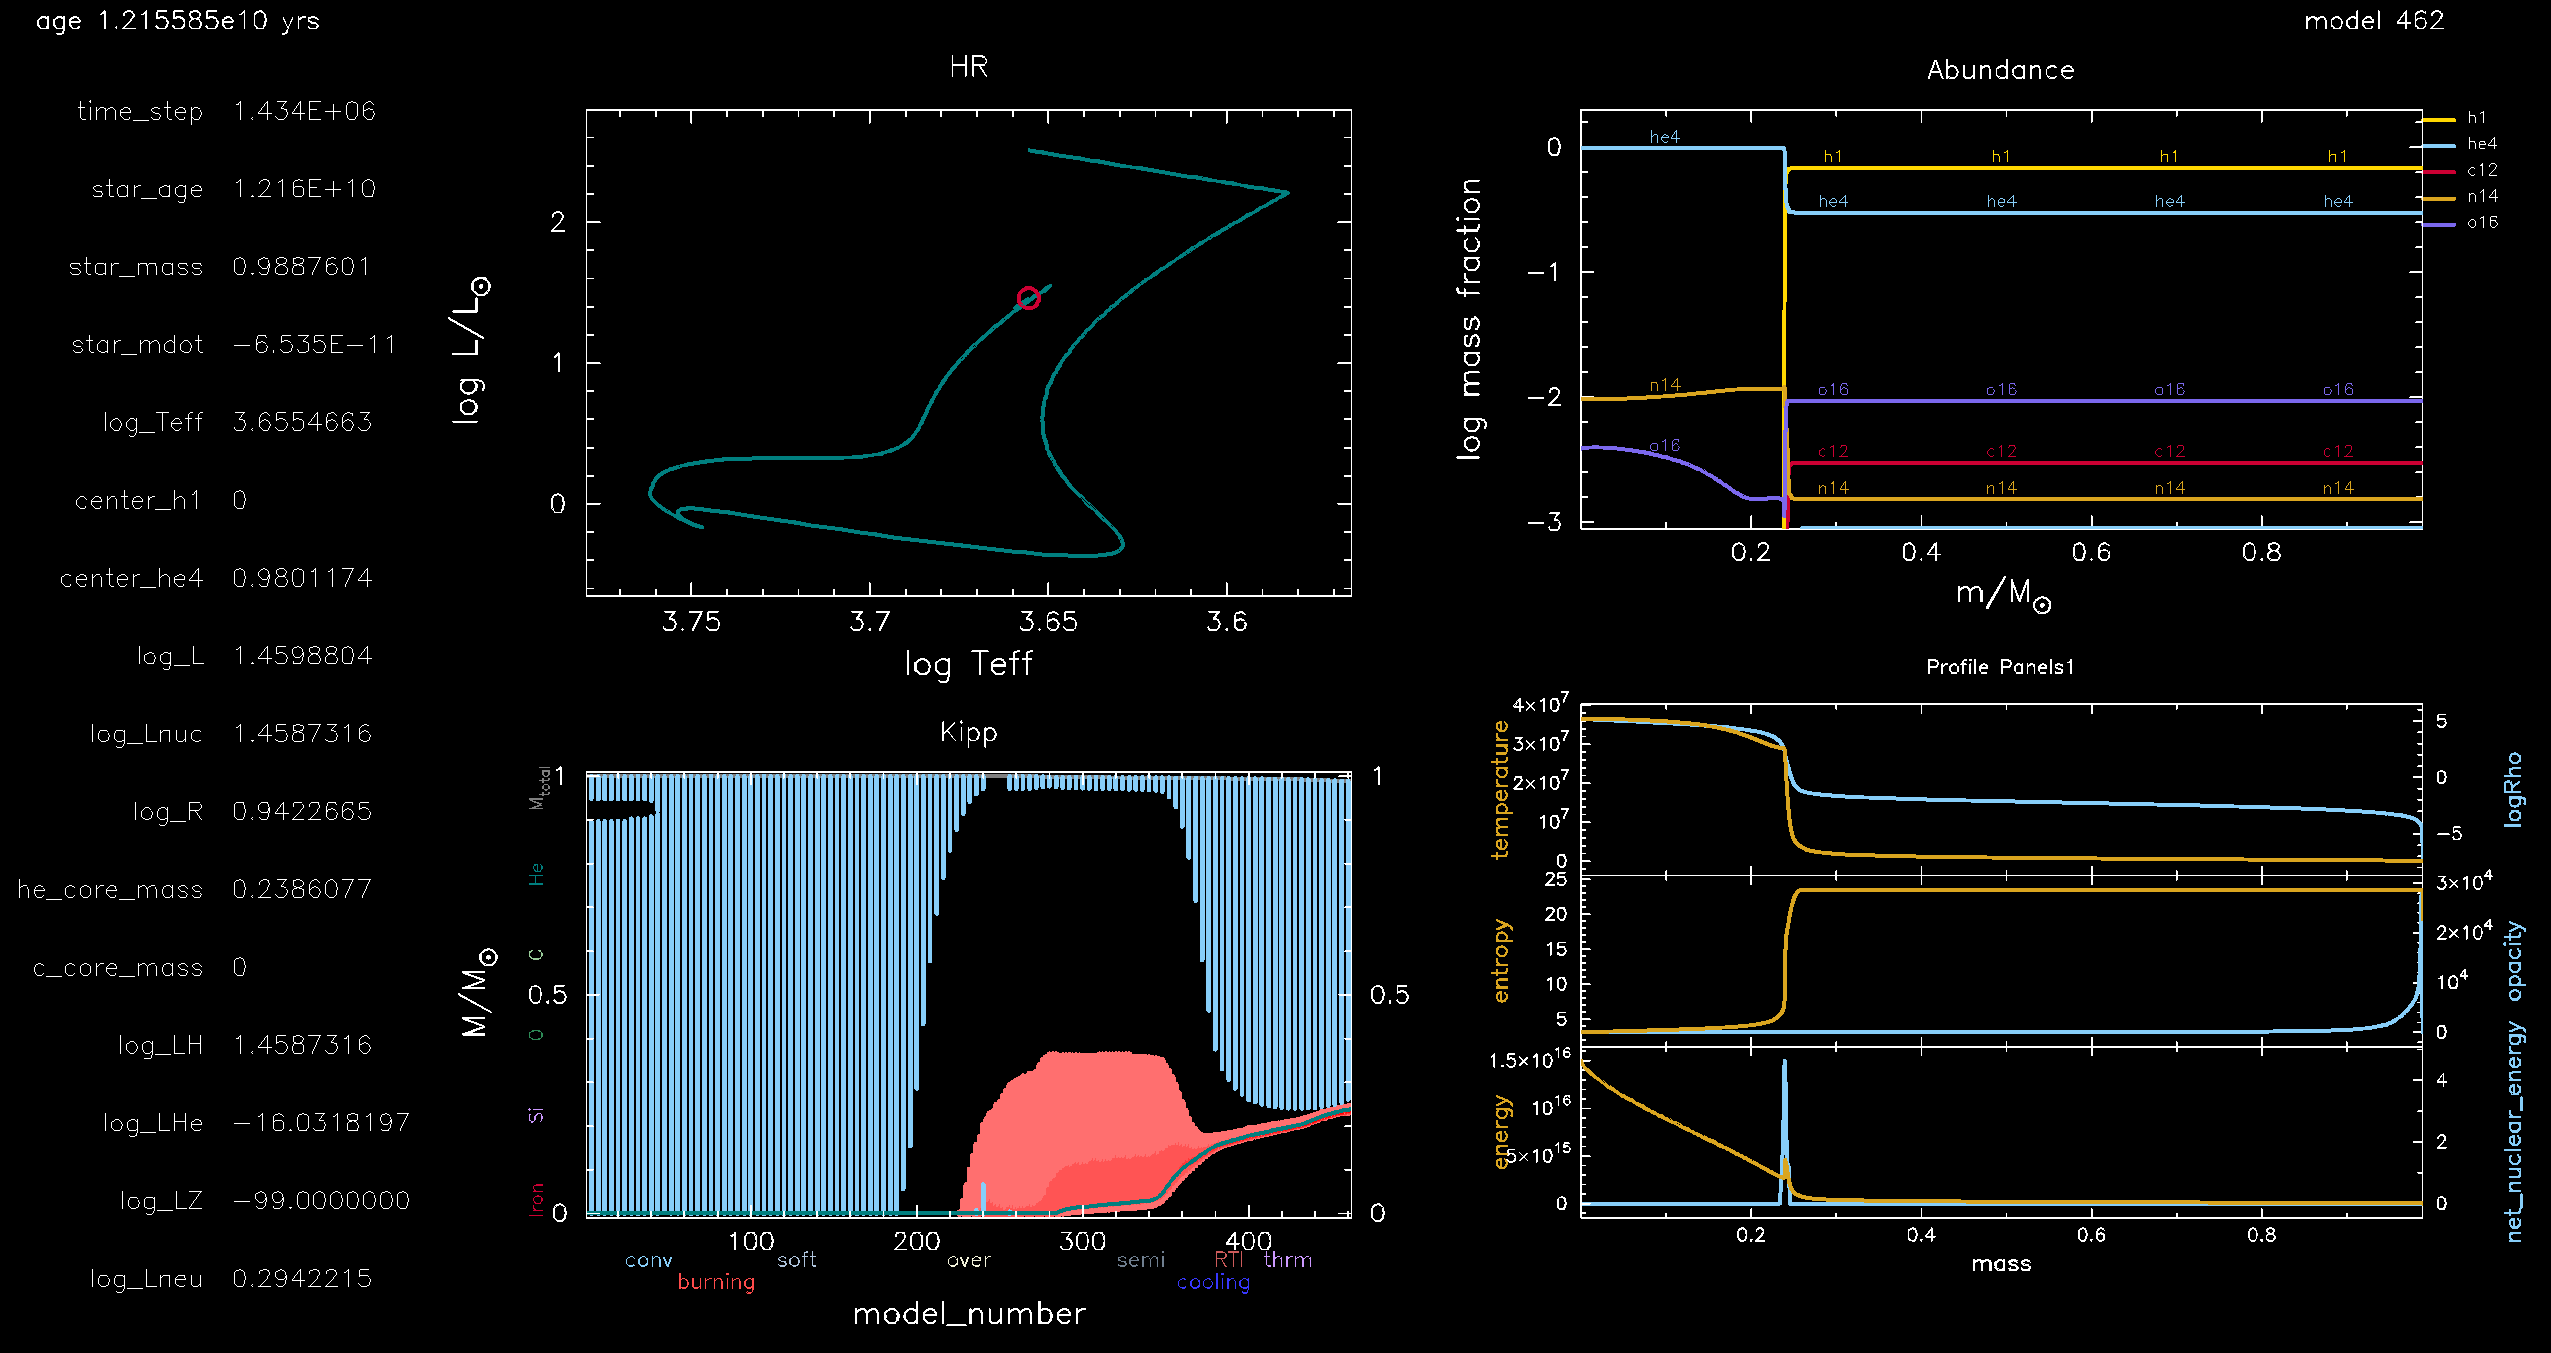
\includegraphics[width=\textwidth]{latex/grid1000462.png}
\caption{The red bump.}
\label{fig:bump}
\end{figure}

\section{GAIA Data}

At the bottom of the notebook, you can plot some higher mass models on the data for the Hyades and Pleiades open clusters.  We will work with them more in the next lab. Here, the data from GAIA gives the absolute magnitude of the stars, and these clusters are so close that reddening is not important, so you can plot the painted models directly on the data without any shifts.

\end{document}
